\documentclass{article}
\usepackage{../fasy-hw}

%% UPDATE these variables:
\renewcommand{\hwnum}{6}
\title{Discrete Structures, Homework \hwnum}
\author{Braeden Hunt (Tinnittin)}
\collab{n/a}
\date{due: 6 April 2021}

\begin{document}

\maketitle

This homework assignment should be
submitted as a single PDF file both to D2L and to Gradescope.

General homework expectations:
\begin{itemize}
    \item Homework should be typeset using LaTex.
    \item Answers should be in complete sentences and proofread.
    \item You will not plagiarize, nor will you share your written solutions
        with classmates.
    \item List collaborators at the start of each question using the \texttt{collab} command.
    \item Put your answers where the \texttt{todo} command currently is (and
        remove the \texttt{todo}, but not the word \texttt{Answer}).
\end{itemize}


% ============================================
% ============================================
\collab{n/a} \nextprob{Applications}
% ============================================
% ============================================

The topics in this class are mathematical in nature, but have strong ties to
computer science: either for understanding how computers work, why algorithms are
correct, or for how to convert real-world data into things that can be analyzed
using a computer.  Explain how each of the following tie to computer science or
data science:

\begin{enumerate}

    \item Tree (be sure that your answer needs a tree, and not a general graph)

        \paragraph{Answer}

        Trees are very useful in computer science to show relationships and to store/search for data efficiently. For example, object oriented programming uses the concepts of parents and children objects, where each child object has a parent object, going all the way back to a base object. This can be represented with a tree. You can see if a object A inherits from another object B if A is in one of B's branches. We can also store a list of data in a tree. By implementing a binary search tree (a tree where each node N has a left and right subtree and every node in the left subtree is less than N and every node that is greater than N is in the right subtree.),  we can quickly search for items within the list.

    \item Directed Graph

        \paragraph{Answer}

       Directed graphs are very useful for handling asymmetric relationships between two nodes. This means that if $(x, y) \in R$ then $(y, x) \in R \iff x=y$. A real world application of this is street maps. Each location can be a node in a directed graph. Each street can be represented by edges in a directed graph. One way streets are represented as single directed edges, and two way streets are represented by two directed edges pointing opposite of each other. So, computer science apllications such as Google Maps can utilize directed graphs to handle street maps.

    \item Equivalence Classes

        \paragraph{Answer}

        Two objects belong to the same equivalence class if they are equivalent to each other. In order for a relationship $R$ to be an equivalence relationship, three properties must to met. $R$ must be reflexive, meaning that $(a,a) \in R$. $R$ is symmetric, meaning that $(a,b) \in R \implies (b,a) \in R$. And $R$ is transitive, meaning if $(a,b) \in R$ and $(b,c) \in R$ then $(a,c) \in R$. In computer science, we often create our own data structures, objects, and classes, and we need to be able to compare them with each other. For example, in Java, we create an ``a.equals(b)'' method. We need to ensure that this only returns true when $a$ and $b$ belong to the same equivalence class so we need to know the properties that need to be met.
        
    \item Distance Metrics

        \paragraph{Answer}

        Distance metrics are ways of defining distances between two different objects. The most common distance metric is Euclidean distance, with the classic $d(P_1, P_2) = \sqrt{(x_2-x_1)^2+(y_2-y_1)^2}$. This is very useful in physics simulations and computational graphics. Another distance metric is the Manhattan Distance, defined as $d(P_1, P_2) = |x_2-x_1|+|y_2-y_1|$, which can be used to represent the distance between two points on city blocks, so it has ties to mapping, just like directed graphs. A more unique and ``nontraditional'' distance metrics is the Damerau–Levenshtein distance, which can be used to measure the distance between strings of characters. This has applications in auto-correct and spell checking suggestions, as an algorithm can identify that a word is misspelled and then compare it to words in a dictionary. It can then suggest words that are close to the misspelling for the user to choose from.


    \item Injective Function

        \paragraph{Answer}

        An injective function is a relationship where every x in the domain maps to a unique y in the co-domain. This means that no two x values maps to the same y value. An example of this in computer science is database tables. A table is full of rows (records) and columns (attributes). Each row is unique and has it's own unique primary key. In this application, the set of all primary keys is the domain, and the set of all rows (the table) is the co-domain. Since each row has it's own unique primary key, the function that maps primary keys to rows is injective. This allows for rows to be referred to by just their primary keys, reducing redundant data, and improving both computational and memory efficiency.


\end{enumerate}


% ============================================
% ============================================
\collab{n/a} \nextprob{Distance Functions}
% ============================================
% ============================================

Suppose you maintain a database of cocktail recipes.  You want to write a
application that asks a user for their favorite cocktail and returns a cocktail
that they might like.  To do so, you define the distance between two cocktails
to be the symmetric distance between their ingredient lists.  Then, for the
input cocktail, you compute the distance to every cocktail in your database and
return one of the cocktails that minimizes this distance.

\begin{enumerate}

    \item Prove that this distance is a metric. (Note: first, formally write out
        what the distance function is, including the domain and codomain).

        \paragraph{Answer}
        $D_{cocktail}(A, B) = max(|\{ i \in A \mid i \notin B\}|, |\{ i \in B \mid i \notin A\}|)$
       
       $D_{cocktail}(A, B)\colon I\times I\to \mathbb{Z}^{nonneg}$ where $A, B \subseteq I$ 
       and $I$ is defined as the set of all ingredients. This means that the domain of $D_{cocktail}$ is the Cartesian product $I\times I$ and the codomain is $\mathbb{Z}^{nonneg}$.
       
       In order to prove that this is a metric, we need to show three things:
       \begin{enumerate}
       
       \item $D_{cocktail}(A, B) \geq 0$
       
       Since $D_{cocktail}(A, B)$ is defined as the max between the size of two sets, and the size of all sets is nonnegative, we know $D_{cocktail}(A, B)$ is greater than or equal to zero.
       
       \item $D_{cocktail}(A, B) = D_{cocktail}(B, A)$
       
       We need to show that  $D_{cocktail}(A, B) = max(|\{ i \in B \mid i \notin A\}|, |\{ i \in A \mid i \notin B\}|) = D_{cocktail}(B, A)$
       
       We start with the definition:  $D_{cocktail}(A, B) =max(|\{ i \in A \mid i \notin B\}|, |\{ i \in B \mid i \notin A\}|)$
       
       By the symmetric property of the $max()$ function, we can switch the order of the two parameters.
       
       Doing so gives us:  $D_{cocktail}(A, B) = max(|\{ i \in B \mid i \notin A\}|, |\{ i \in A \mid i \notin B\}|)$ 
       
       Since $max(|\{ i \in B \mid i \notin A\}|, |\{ i \in A \mid i \notin B\}|) = D_{cocktail}(B, A)$, we have shown what was to be shown.
       
       \item $D_{cocktail}(A, B) \leq D_{cocktail}(A, C) + D_{cocktail}(C, B)$
       
       Let's break  $D_{cocktail}(A, B)$ down into two cases.
       \begin{enumerate}
       \item Case 1: $|A| \leq |B|$:
       
       Then $D_{cocktail}(A, B) = |\{ i \in B \mid i \notin A\}|$.
       
       $D_{cocktail}(A, C) = |\{ i \in C \mid i \notin A\}|$.
       
       $D_{cocktail}(C, B) = |\{ i \in B \mid i \notin C\}|$.
       
	$D_{cocktail}(A, C) + D_{cocktail}(C, B) = |\{ i \in C \mid i \notin A\}| + |\{ i \in B \mid i \notin C\}|$
	
	$= |\{ i \in C \mid i \notin A \land i \notin B\}| +  |\{ i \in C \mid i \notin A \land i \in B\}| + |\{ i \in B \mid i \notin C \land  \notin A\}| + |\{ i \in B \mid i \notin C \land  \in A\}|$ 
	\qquad by splitting sets into disjoint sets that sum together to the original.
       
       We can rewrite $|\{ i \in C \mid i \notin A \land i \in B\}|$ as $|\{ i \in B \mid i \notin A \land i \in C\}|$.
       
       We can then combine that term with $ |\{ i \in B \mid i \notin C \land  \notin A\}|$ to get $ |\{ i \in B \mid i \notin A\}|$ which equals $D_{cocktail}(A, B)$.
       
       This gives us $D_{cocktail}(A, C) + D_{cocktail}(C, B) = D_{cocktail}(A, B) + |\{ i \in B \mid i \notin C \land  \in A\}| + |\{ i \in C \mid i \notin A \land i \notin B\}|$.
       
       Since $D_{cocktail}(A, C) + D_{cocktail}(C, B)$ is equal to $D_{cocktail}(A, B) + x$ where x is some nonnegative integer, we know  $D_{cocktail}(A, B) \leq D_{cocktail}(A, C) + D_{cocktail}(C, B)$
       
        \item Case 2: $|B| \leq |A|$:
       
       Then $D_{cocktail}(A, B) = |\{ i \in A \mid i \notin B\}|$.
       
       $D_{cocktail}(A, C) = |\{ i \in C \mid i \notin A\}|$.
       
       $D_{cocktail}(C, B) = |\{ i \in B \mid i \notin C\}|$.
       
	$D_{cocktail}(A, C) + D_{cocktail}(C, B) = |\{ i \in A \mid i \notin C\}| + |\{ i \in C \mid i \notin B\}|$
	
	$= |\{ i \in C \mid i \notin A \land i \notin B\}| +  |\{ i \in C \mid i \notin B \land i \in A\}| + |\{ i \in A \mid i \notin C \land  \notin B\}| + |\{ i \in A \mid i \notin C \land  \in B\}|$ 
	\qquad by splitting sets into disjoint sets that sum together to the original.
       
       We can rewrite $|\{ i \in C \mid i \notin B \land i \in A\}|$ as $|\{ i \in A \mid i \notin B \land i \in C\}|$.
       
       We can then combine that term with $ |\{ i \in A \mid i \notin C \land  \notin B\}|$ to get $ |\{ i \in A \mid i \notin B\}|$ which equals $D_{cocktail}(A, B)$.
       
       This gives us $D_{cocktail}(A, C) + D_{cocktail}(C, B) = D_{cocktail}(A, B) + |\{ i \in A \mid i \notin C \land  \in B\}| + |\{ i \in C \mid i \notin B \land i \notin A\}|$.
       
       Since $D_{cocktail}(A, C) + D_{cocktail}(C, B)$ is equal to $D_{cocktail}(A, B) + x$ where $x$ is some nonnegative integer, we know  $D_{cocktail}(A, B) \leq D_{cocktail}(A, C) + D_{cocktail}(C, B)$
       
       \end{enumerate}
       \end{enumerate}
        
    \item Is this a good distance to use for your application?  Why or why not?

        \paragraph{Answer}

        This is not a good distance metric because it does not take into account other factors that affect taste. The biggest one is the quantity of each ingredient. 
        Since this metric doesn't include that in the measure, Cocktail A with 10 x ingredient and 1 y ingredient would be equal to Cocktail B with 10 y ingredient and 1 x ingredient. These two would not taste at all similar, 
        but this distance metric would say they should taste exactly the same.

\end{enumerate}


% ============================================
% ============================================
\collab{n/a} \nextprob{Loop Invariant}
% ============================================
% ============================================

Recall that a loop invariant is used to prove that a loop is correct (which in
turn helps to prove that an algorithm is correct).

\begin{enumerate}

    \item Write pseudocode that uses a while loop to find the second largest
        element in an unsorted array.  The input to your algorithm should be an
        unsorted array $A$ of real values.  The psuedocode should use the
        variable name \textsc{curguess} to store the current guess of the second
        largest value, and \textsc{curmax} to store the current max of $A$.

        \paragraph{Answer} Algorithm:

        secondMax(array A)
        
        \qquad if (A[1] > A[2])
        
        \qquad \qquad curmax = A[1]
       
        \qquad \qquad curguess = A[2]
        
        \qquad else 
       
        \qquad \qquad curmax = A[2]
       
        \qquad \qquad curguess = A[1]
        
        \qquad i = 3
       
        \qquad while i $\leq$ A.length
       
        \qquad \qquad if A[i] $>$ curmax
       
        \qquad \qquad \qquad curguess = curmax
       
        \qquad \qquad \qquad curmax = A[i]
        
        \qquad \qquad else if A[i] $>$ curguess and curmax $>$ A[i]
        
        \qquad \qquad \qquad curguess = A[i]
        
        \qquad \qquad i = i + 1
        
        \qquad return curguess
        

    \item What is the postcondition of the loop? (Call this statement $Q$).

        \paragraph{Answer}

        $Q\colon$ the value returned is the second greatest in the array.

    \item What is the precondition of the loop? (Call this statement $P$).

        \paragraph{Answer}

       $P\colon$ A is an array of real values, i = 3, curmax equals the max of the first two elements of A, and curguess equals the minimum of the first two elements of A

    \item What is the loop guard of the loop? (Call this statement $G$).

        \paragraph{Answer}

        $G\colon i \leq A.length$

    \item Prove that the loop invariant is when entering the $i^\text{th}$
        iteration of the loop is, ``the variable \textsc{curguess} stores
        the second
        largest value of $A[1,2, \ldots, i]$,
        and \textsc{curmax} stores the largest value of $A[1,2,\ldots, i]$.

        \paragraph{Answer}
\begin{enumerate}
	\item Basis Property: $P$ is true.
	
	A is an array of real values is true (given by the problem). i=3 because we set it to that. curmax is the largest value in the first two elements of the array and curguess is the second greatest value (also the minimum value) of the array as it is the only other value besides curmax.
	
	\item Inductive Property: If $G \land I(k)$ is true before a loop iteration (where $k \geq 0$), then $I(k+1)$ is true after the loop iteration.
	
	We assume that $G \land I(k)$ is true. That means $i = k+3$, curmax is eqaul to the greatest value in A[1, 2, ..., ($i-1$)], and curguess holds the second greatest value in that same range.
	
	The $k+1$ iteration of the loop starts by comparing A[i] to curmax and curguess. There are three possible cases:
	
	\begin{enumerate}
	\item A[i] is the max of A[1, 2, ..., i]:
	
	A[i] is greater than curmax, so the first if-statement block executes. This means curmax is now the second largest value so curguess is updated to that value. 
	The new max is A[i] so curmax is set to that value. The loop then increments i so the next iteration is $I(i+1)$.
	
	\item A[i] is the second greatest value in A[1, 2, ..., i]
	
	A[i] is less than the curmax, but is greater than the curgess, so the second if-statement block executes. This means that curguess is updated to A[i]. 
	Curmax does not need to be updated as it is still the max of the first i elements of A. The loop then increments i so the next iteration is $I(i+1)$.
	
	\item A[i] is not the maximum or second greatest value of A[1, 2, ..., i].
	
	Curguess and curmax do not get updated as neither if-statement is triggered.  The loop then increments i so the next iteration is $I(i+1)$.
\end{enumerate}


	In all possible cases, the loop invariant holds, as was to be shown.
\end{enumerate}
\end{enumerate}



% ============================================
% ============================================
\collab{n/a} \nextprob{Four Colors Suffice}
% ============================================
% ============================================

Read Chapters $9$ and $10$ of \emph{Four Colors Suffice}.

\begin{enumerate}

    \item What is a \emph{reducible configuration}?

        \paragraph{Answer}

        A part of a map, or submap, that cannot exist within a minimal criminal. This means that if a map has a reducible configuration within it, it can be ruled out for needing to be checked to see if it can be colored. This allowed Appel and Haken to speed up their computer program.



    \item Who was the first to correctly prove the four color theorem?  What
        role did computers play in the proof?

        \paragraph{Answer}

        Kenneth Appel and Wolfgang Haken were the first to solve the problem. They used computers to construct a unavoidable set of reducible configurations. 
        This means that every map must have at least one of the reducible configurations within it. Because every map contains an reducible configuration, then every map can be
        colored with four colors.




    \item Draw a ``map'' on the M\"obius strip that requires five or more colors
        to color.

        \paragraph{Answer}
        See Figure \ref{mobius}

        \begin{figure}
\caption{Mobius Strip map that requires five or more colors}
\centering
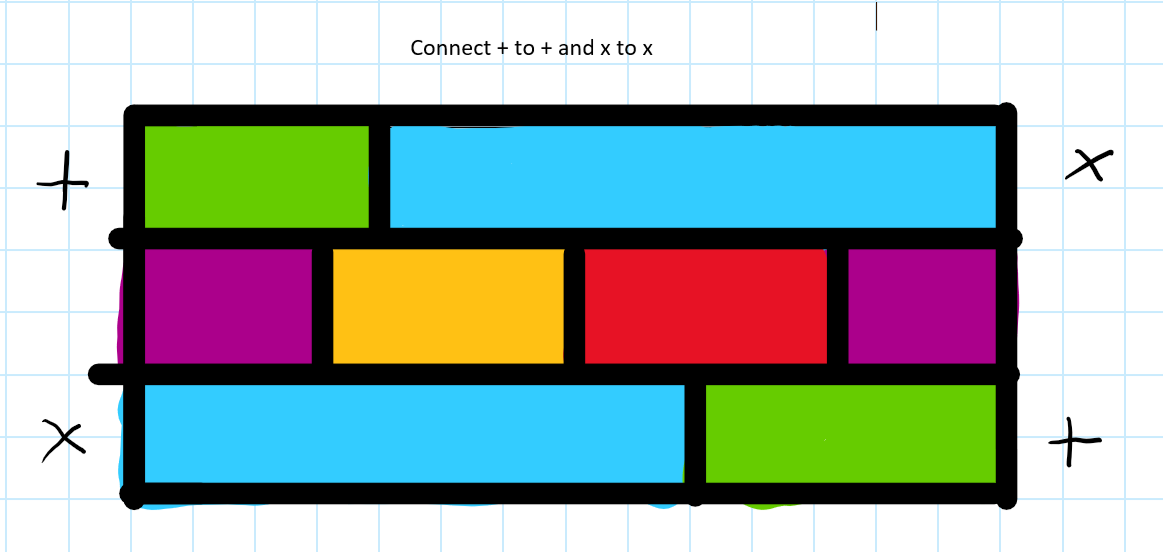
\includegraphics[width=\textwidth]{images/mobius}
\label{mobius}
\end{figure}


\end{enumerate}

% ============================================
% ============================================
\collab{n/a}
\nextprob{Shafi Goldwasser}
% ============================================
% ============================================

Write a short (1-2 paragraph) biography of Shafi Goldwasser.
\textbf{In your own words}, describe who they are and why they are important in
the history of computer science.

If you use external resources, please provide
proper citations. If you do not use external sources, please write ``I did not
use any sources to write this biography'' as the last sentence of the
biography.

\paragraph{Answer}

Shafi Goldwasser was born in New York City in 1959 and had dual citizenship with Israel as her parents were Israeli. She grew up in Israel and later attended Cambridge studying mathematics. She soon started programming and attended graduate school at Berkeley. She created methods of encrypting a single bit, which allowed creating a secure message of many bits. After graduating, she moved to MIT as a postdoc and later a faulty member. There, she continued to work in the field of cryptography, making large advances and even creating new methods of proofs that utilize computers. She went on to become an A.M. Turing Award Laureate and won the Gödel Prize, along with a whole host of other major awards.

Source: Shafi Goldwasser. (2012). Retrieved April 04, 2021, from \url{https://amturing.acm.org/award_winners/goldwasser_8627889.cfm}

% %% ... the bibliography
% \newpage
% \bibliographystyle{acm}
% \bibliography{biblio}

\end{document}

